\documentclass{article}
\usepackage{amsmath}
\usepackage[utf8]{inputenc}
\usepackage{float}
\usepackage{epsfig,graphicx}
\usepackage{xcolor,import}
\usepackage[german]{babel}

\begin{document}


\thispagestyle{empty}
			\begin{center}
			\Large{Fakultät für Physik}\\
			\end{center}
\begin{verbatim}


\end{verbatim}
							%Eintrag des Wintersemesters
			\begin{center}
			\textbf{\LARGE WINTERSEMESTER 2014/15}
			\end{center}
\begin{verbatim}


\end{verbatim}
			\begin{center}
			\textbf{\LARGE{Physikalisches Praktikum 1}}
			\end{center}
\begin{verbatim}




\end{verbatim}

			\begin{center}
			\textbf{\LARGE{PROTOKOLL}}
			\end{center}
			
\begin{verbatim}





\end{verbatim}

			\begin{flushleft}
			\textbf{\Large{Experiment (Nr., Titel):}}\\
							%Experiment Nr. und Titel statt den Punkten eintragen
			\LARGE{1. Messen - Messfehler}	
			\end{flushleft}

\begin{verbatim}

\end{verbatim}	
							%Eintragen des Abgabedatums, oder des Erstelldatums des Protokolls
			\begin{flushleft}
			\textbf{\Large{Datum:}} \Large{17.10.2014}
			\end{flushleft}
			
\begin{verbatim}
\end{verbatim}
							%Namen der Protokollschreiber
		\begin{flushleft}
			\textbf{\Large{Namen:}} \Large{Veronika Bachleitner, Erik Grafendorfer}
			\end{flushleft}

\begin{verbatim}


\end{verbatim}
							%Kurstag und Gruppennummer, zb. Fr/5
			\begin{flushleft}
			\textbf{\Large{Kurstag/Gruppe:}} \Large{Fr/1}
			\end{flushleft}

\begin{verbatim}






\end{verbatim}
							%Name des Betreuers, das Praktikum betreute.
			\begin{flushleft}
			\LARGE{\textbf{Betreuer:}}	\Large{SETMAN}	
			\end{flushleft}
%		\begin{figure}[!h]
%\def\svgwidth{70mm}
%\import{section1/}{nonne.eps_tex}
%\end{figure}
%$\pm$
%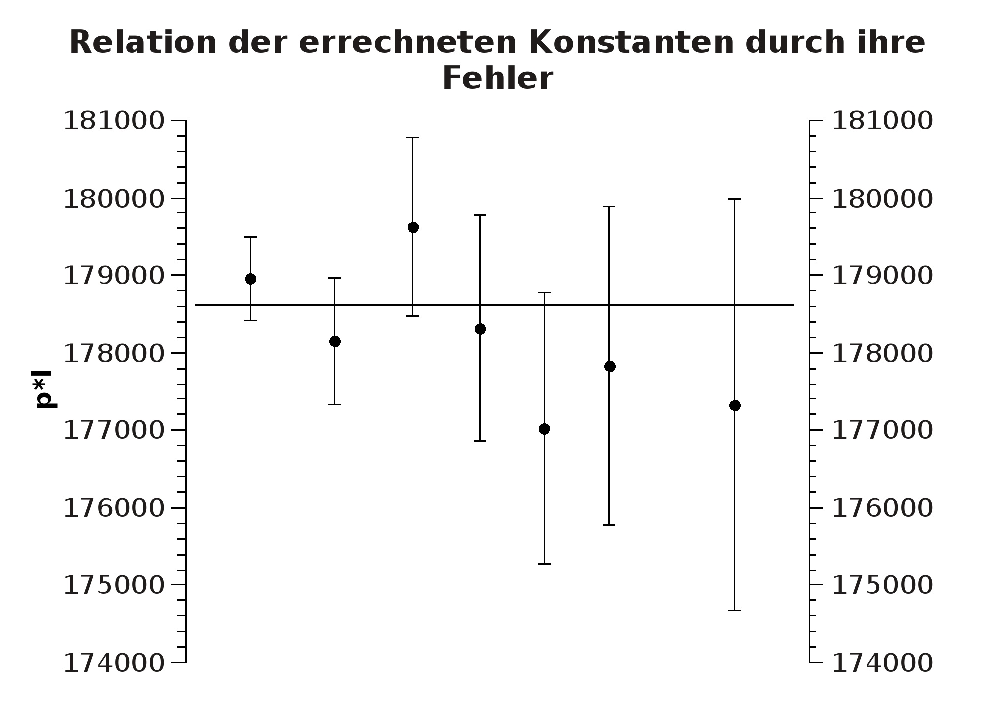
\includegraphics[scale=1,angle=-90]{Graph1.eps}[!h]
\section{Pendel}	
\subsection{Aufgabenstellung}
Es soll die Erdbeschleunigung aus Messungen der Periodendauer eines einfachen Fadenpendels bestimmt werden. Dazu werden 2 Messreihen durchgeführt: Einmal 10 Einzelmessungen als Messreihe; einmal eine Messung von 10 aufeinander folgenden Schwingungen.
\subsection{Grundlagen zum Experiment}
Das Fadenpendel stellt die experimentelle Näherung an ein mathematisches Pendel dar. Bei einem mathematischen Pendel ist die gesamte Masse im Schwerpunkt, die Aufhängung ist starr und reibungsfrei, sowie masselos.
\subsubsection*{Berechnung der Erdbeschleunigung}
Aus der Schwingungsdauer des Pendels können wir uns die lokale Erdbeschleunigung g näherungsweise berechnen. Wir verwenden für kleine Auslenkungswinkel $\alpha$ die Näherung Sin[$\alpha$] $\approx$ $\alpha$. 
Für die Schwingungsdauer T, die Frequenz f und die Pendellänge l gilt:

\begin{align}
T=\frac{1}{f}=2 \pi\sqrt{\frac{l}{g}} \\
g=4\pi^2\frac{l}{T^2}
\end{align}
\subsection{Material und Methoden / Versuchsaufbau}

\subsection{Durchführung des Experiments}

\subsection{Ergebnisse}
Wir berechnen die Unsicherheit der Erdbeschleunigung $\Delta g$ in Abhängigkeit von den gemessenen Größen laut dem Gaußschen Fehlerfortpflanzungsgesetz. Wir berechnen diese 2 Mal, nachdem wir unterschiedliche Näherungswerte und Unsicherheiten für die Schwingungsdauer erhalten wenn wir sie 10 Mal einzeln oder 10 Mal in Folge messen.
\begin{align}
\Delta g=\sqrt{(\frac{\delta g}{\delta l})^2\Delta l^2 + (\frac{\delta g}{\delta T})^2\Delta T^2}
\end{align} \\
Für die 10 Einzelmessungen ist
\begin{equation}
T_{Einzel,genaehert} = (1.93 \pm 0.02)s
\end{equation}
Damit:
\begin{equation}
\Delta g_{Einzel,genaehert} = 0.067 \frac{m}{s^2}
\end{equation}


\begin{equation}
T_{Serie,genaehert} = (1.94 \pm 0.01)s
\end{equation}
Damit:
\begin{equation}
\Delta g_{Serie,genaehert} = 0.0376 \frac{m}{s^2}
\end{equation}
\begin{table}
\caption{Messungen einzelner Schwingungen}
\begin{center}
\begin{tabular}{|c|c|}
\hline \\
Durchgang & Schwingungsdauer[($\pm$0.02s)]\\
\hline 1&1.96\\
\hline 2&1.93\\
\hline 3&1.87\\
\hline 4&1.95\\
\hline 5&1.82\\
\hline 6&1.93\\
\hline 7&1.92\\
\hline 8&1.99\\
\hline 9&1.9\\
\hline 10&1.97\\
\hline

\end{tabular} \\
\vspace{1cm}
Messung von 10 konsekutiven Schwingungen:\\
\vspace{1cm}
$T_{Serie}$=(19.36 $\pm$0.01)s
\end{center}
\end{table}

Wir verwenden die genauesten Paare von Pendellänge und Schwingungsdauer von allen drei Gruppen, plus einem Paar, das uns die Praktikumsleiterin zur Verfügung stellte, um eine lineare Regression über die Pendellängen durch die Quadrate der Schwingungsdauern zu fitten. Wir verwendeten QtiPlot 0.9.8.9 für die Berechnung und die Darstellung. \\
\begin{figure}


\centering
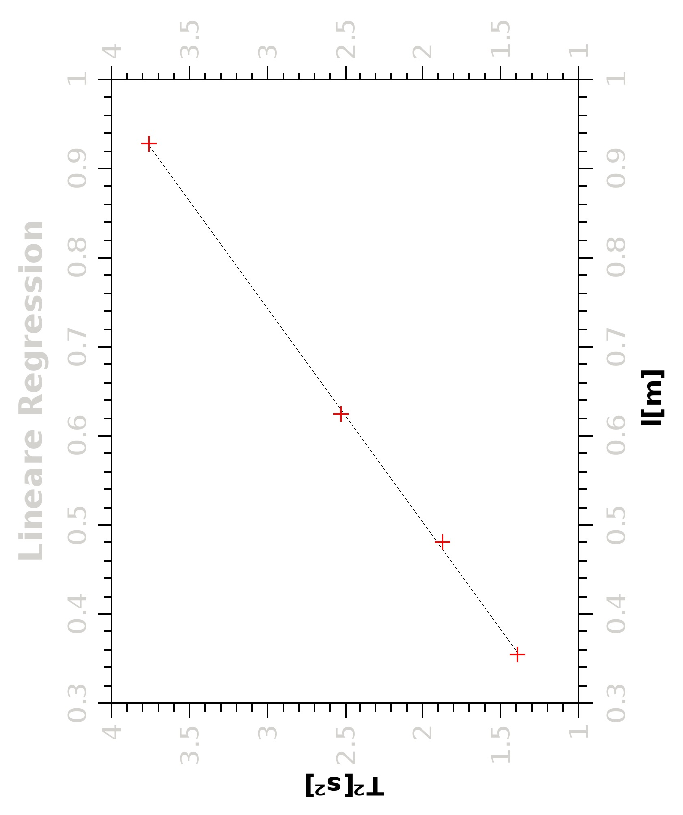
\includegraphics[scale=0.8,angle=-90]{LinearReg.eps} \\
\includegraphics[scale=0.5,angle=0]{regressiondata.eps}
\caption{Lineare Regression}

\end{figure}
\subsection{Diskussion}
\section{Mechanische Messungen}
\subsection{Aufgabenstellung}
Es soll der Durchmesser eines Kupferdrahtes mit verschiedenen Methoden gemessen werden. Verwendet werden eine Schublehre, eine Mikrometerschraube und ein Mikroskop mit Okularmaßstab.\\
Ferner sollen 3 Winkel eines Metall-Dreiecks mit einer Winkellehre gemessen werden.

\subsection{Grundlagen zum Experiment}
\subsubsection*{Schublehre}
Mit der Schublehre können Längen mit einer Genauigkeit von 0,05mm gemessen werden. Es gibt eine Hauptskala in Millimeter sowie einen Nonius auf einem beweglichen Schieber. Auf der verwendeten Schublehre sind 20 Teile der Noniusskala auf 39mm der Hauptskala aufgeteilt. Das bedeutet, dass 1mm durch 20 geteilt wird und wir somit die besagte Genauigkeit von $\pm$0,05mm erhalten.\\
%Das hast du so gut beschrieben, Vero, dass ich den Ruf nach einer Abbildung im Äther verhallen lasse.
\subsubsection*{Mikrometerschraube}
Mit der Mikrometerschraube können Längen mit einer Genauigkeit von $\pm$0,01mm gemessen werden.

\subsubsection*{Mikroskop}
Am Mikroskop verwenden wir das OBJEKTIV?? und einen geeichten Maßstab von 2mm Länge mit Genauigkeit $\pm$0.01mm um die Dicke des Drahtes noch genauer messen zu können. 
\subsubsection*{Winkellehre}
Um mit der Winkellehre zu messen legt man das zu messende Objekt zwischen die beiden Mess-Schenkel und passt die Schenkel an die Größe an. Das Ergebnis ist wie bei der Schublehre an einer Hauptskala mit Nonius abzulesen.

\subsection{Material und Methoden / Versuchsaufbau}

\subsection{Durchführung des Experiments}

\subsection{Ergebnisse}

\begin{table}
\centering
\begin{tabular}{|c|c|c|}
\hline
n&$l_1$[mm]&$l_2$[mm]\\
\hline
\hline
1&0.25&0.2\\
2&0.2&0.21\\
3&0.25&0.2\\
4&0.2&0.2\\
5&0.25&0.2\\
\hline 
$\bar{l}$&0.23&0.20\\
\hline
\end{tabular}
\caption{Messungen mit der Schublehre und der Mikrometerschraube}
\end{table}

Wir messen die Dicke des Kupferdrahtes an verschiedenen Stellen  fünf Mal mit der Schublehre, fünf Mal mit der Mikrometerschraube und ein Mal mit dem Mikroskop.  Die Messungenauigkeit der Schublehre liegt mit 0.05mm über dem Standardfehler von 0.012mm, darum ist die Länge hier

\begin{equation}
l_1=(0.23\pm0.05)mm
\end{equation}
\\
Bei der Mikrometerschraube ist die Messungenauigkeit mit 0.1mm ebenfalls größer als der Standardfehler der Messungen von 0.001mm, also ist hier \\ 
\begin{equation}
l_2=(0.2\pm0.1)mm. 
\end{equation}
Die Messung mit dem Mikroskop ergab eine Länge $l_3$ von
\begin{equation}
l_3=(0.19 \pm 0.01) mm
\end{equation}
Nachdem wir mit drei verschiedenen Instrumenten in unseren Augen gut gemessen haben, wollen wir noch ein gewichtetes Mittel aus diesen drei Ergebnissen ermitteln um all unsere Messungen in das Endergebnis einfließen zu lassen. Dabei verwenden wir für die Gewichtungsfaktoren:
\begin{equation}
\frac{1}{\Delta l_1}+\frac{1}{\Delta l_2}+\frac{1}{\Delta l_3}=g_1:g_2:g_3=20:10:100=2:1:10
\end{equation}
Nun:
\begin{gather*}
\bar{l_g}=\frac{\bar{l_1}g_1+\bar{l_2}g_2+\bar{l_3}g_3}{g_1+g_2+g_3} \\
\bar{l_g}=\frac{0.23\cdot2+0.2\cdot1+0.19\cdot10}{2+1+10} \\
\bar{l_g}=0.197mm \\
\Delta l_g= \sqrt{\frac{\Sigma^k_{j=1}( \bar{l_j} -\bar{l_g} )^2 \cdot g_j}{(k-1)\Sigma^k_{j=1}g_j} } \\
\Delta l_g= \sqrt{\frac{(0.23-0.197)^2\cdot2+(0.20-0.197)^2\cdot1+(0.19-0.197)^2\cdot10}{(3-1)(2+1+10)}}\\ = 0.014mm \\
\end{gather*}\\
Unser Endergebnis ist demnach:\\
\begin{equation}
l_g=\bar{l_g}\pm\Delta l_g = (0.197\pm0.014)mm
\end{equation}\\
\subsection{Diskussion}
Die Messergebnisse mit den immer genaueren Instrumenten der Mikrometerschraube, der Schublehre und des geeichten Maßstabs am Mikroskop liegen in schöner Übereinstimmung miteinander, die Mittelwerte der Messergebnisse liegen innerhalb der Konfidenzintervalle der Messungenauigkeiten aller Instrumente. Wir können also mit hoher Wahrscheinlichkeit davon ausgehen dass wir genau gemessen haben.
\section{Elektrische Messungen}
\subsection{Aufgabenstellung}
Im Gleichstrom messen Ströme und Spannungen in verschiedenen Schaltungen, mal spannungsrichtig, mal stromrichtig, um mit Augenmerk auf die Fehlergrenzen unserer Messgeräte zu sehen, ob wir unsere Messungen wegen der Innenwiderstände der Messgeräte überhaupt korrigieren müssen oder nicht.\\
Weiters messen wir in Parallel- und Serienschaltungen Widerstände und vergleichen sie mit den berechneten Werten.\\
Im Wechselstrom bauen wir einen Spannungsteiler und berechnen Spannungen und Ströme auch in einer modifizierten Schaltung mit einem Kondensator.
\\
\subsection{Grundlagen zum Experiment}
Spannung U: [U]=V (Volt)\\
Stromstärke I: [I]=A (Ampère)\\
Widerstand R: [R]=$\Omega$ (Ohm)\\

Das Ohm'sche Gesetz: U=RI

\subsection{Material und Methoden / Versuchsaufbau}
\includegraphics[scale=0.8,angle=-180]{1stromrichtig.eps}

\subsection{Durchführung des Experiments}

\subsection{Ergebnisse}

\subsection{Diskussion}

\end{document}
